\documentclass[tikz,border=6pt]{standalone}
\usepackage{pgfplots}
\pgfplotsset{compat=1.18}
\usepgfplotslibrary{colormaps}
\usetikzlibrary{arrows, arrows.meta, calc}
\usetikzlibrary{decorations.markings}


\usepackage{amssymb,amsmath,mathtools}

\usepackage[T1]{fontenc}
\usepackage[utf8]{inputenc}
\usepackage{newpxtext,newpxmath}
\usepackage{sectsty}

\renewcommand{\Re}{\operatorname{\mathrm{Re}}}
\renewcommand{\Im}{\operatorname{\mathrm{Im}}}

\begin{document}
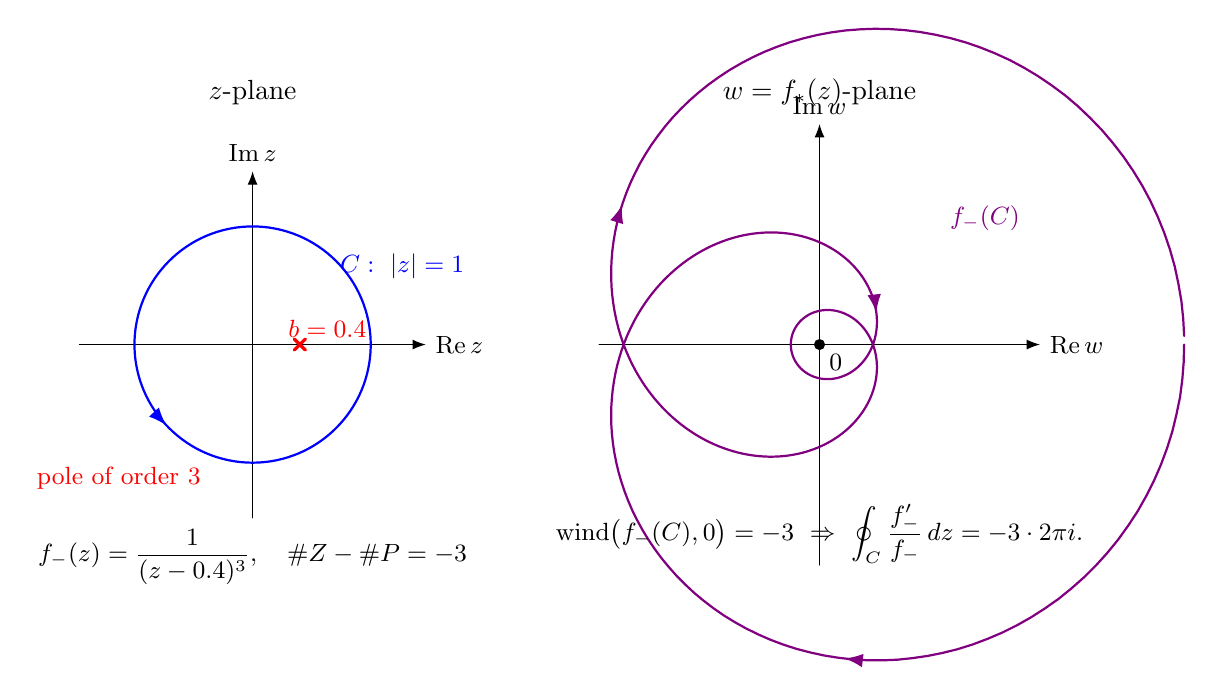
\begin{tikzpicture}[>=Latex, line cap=round, line join=round, font=\small]

% ===== Left: z-plane =====
\begin{scope}
	\node[font=\normalsize] at (0,3.2) {$z$-plane};
	\draw[->] (-2.2,0)--(2.2,0) node[right] {$\Re z$};
	\draw[->] (0,-2.2)--(0,2.2) node[above] {$\Im z$};
	
	% C: unit circle
	\draw[blue,thick,postaction={decorate},
	decoration={markings, mark=at position 0.62 with {\arrow{>}}}]
	(0,0) circle (1.5);
	\node[blue] at (1.9,1.0) {$C:\ |z|=1$};
	
	% triple pole at 0.4
	\draw[red,very thick] (0.6,0) ++(-0.07,-0.07) -- ++(0.14,0.14);
	\draw[red,very thick] (0.6,0) ++(-0.07,0.07) -- ++(0.14,-0.14);
	\node[red] at (0.95,0.2) {$b=0.4$};
	\node[red] at (-1.7,-1.7) {pole of order $3$};
	
	\node[align=left] at (0,-2.7) {$\displaystyle
		f_-(z)=\frac{1}{(z-0.4)^3},\quad \#Z-\#P=-3$};
\end{scope}

% ===== Right: w-plane =====
\begin{scope}[shift={(7.2,0)}]
	\node[font=\normalsize] at (0,3.2) {$w=f_*(z)$-plane};
	\draw[->] (-2.8,0)--(2.8,0) node[right] {$\Re w$};
	\draw[->] (0,-2.8)--(0,2.8) node[above] {$\Im w$};
	\fill (0,0) circle(2pt) node[below right] {$0$};
	
	% Parametrize z = e^{it} = x+iy, x=cos t, y=sin t
	% u = x - 0.4, v = y
	% (u+iv)^3 = P + iQ where
	%   P = u^3 - 3u v^2,  Q = 3u^2 v - v^3
	% 1/(u+iv)^3 = (P - iQ)/(P^2+Q^2)
	\draw[violet,thick,
	postaction={decorate},
	decoration={markings,
		mark=at position 0.18 with {\arrow{>}},
		mark=at position 0.45 with {\arrow{>}},
		mark=at position 0.72 with {\arrow{>}}}]
	plot[domain=0:6.283, samples=650] 
	({
		% Re = P/(P^2+Q^2)
		( ((cos(\x r)-0.4)^3 - 3*(cos(\x r)-0.4)*(sin(\x r))^2 )
		)
		/
		(
		((cos(\x r)-0.4)^3 - 3*(cos(\x r)-0.4)*(sin(\x r))^2 )^2
		+ ( 3*(cos(\x r)-0.4)^2*(sin(\x r)) - (sin(\x r))^3 )^2
		)
	},
	{
		% Im = -Q/(P^2+Q^2)
		( - ( 3*(cos(\x r)-0.4)^2*(sin(\x r)) - (sin(\x r))^3 ) )
		/
		(
		((cos(\x r)-0.4)^3 - 3*(cos(\x r)-0.4)*(sin(\x r))^2 )^2
		+ ( 3*(cos(\x r)-0.4)^2*(sin(\x r)) - (sin(\x r))^3 )^2
		)
	});
	\node[violet] at (2.1,1.6) {$f_-(C)$};
	
	\node[align=center] at (0,-2.4)
	{$\mathrm{wind}\big(f_-(C),0\big)=-3
		\ \Rightarrow\ 
		\displaystyle \oint_C \frac{f_-'}{f_-}\,dz=-3\cdot 2\pi i.$};
\end{scope}

\end{tikzpicture}
\end{document}
